\pagestyle{fancy}
% 页眉页脚设置
\pagenumbering{arabic}\setcounter{page}{1}
\lhead{\song \fontsize{9pt}{13pt}\selectfont 兰州大学研究生毕业论文\LaTeX 模板 }
\chead{}
\rhead{\song \fontsize{9pt}{13pt}\selectfont \selectfont 兰州大学研究生毕业论文\LaTeX 模板}
\lfoot{}
\cfoot{\thepage}
\rfoot{}


\section*{第一章~~介绍}
\setcounter{section}{1} \setcounter{subsection}{0}
\addcontentsline{toc}{section}{第一章~~介绍}

\subsection{参考文献示例}
\par 文章FullyConvolutionalNetwork\upcite{FCN_}.
\par 多篇文章引用示例\upcite{FCN_,ronneberger2015u,ref8-1,ref8-2}。
\subsection{图像插入示例}
\par 图像位置在本项目的Img文件夹下,可以点上传后同本地上传,建议按照章节命名编号,便于保存.
\begin{figure}[!htbp]
    \centering    
    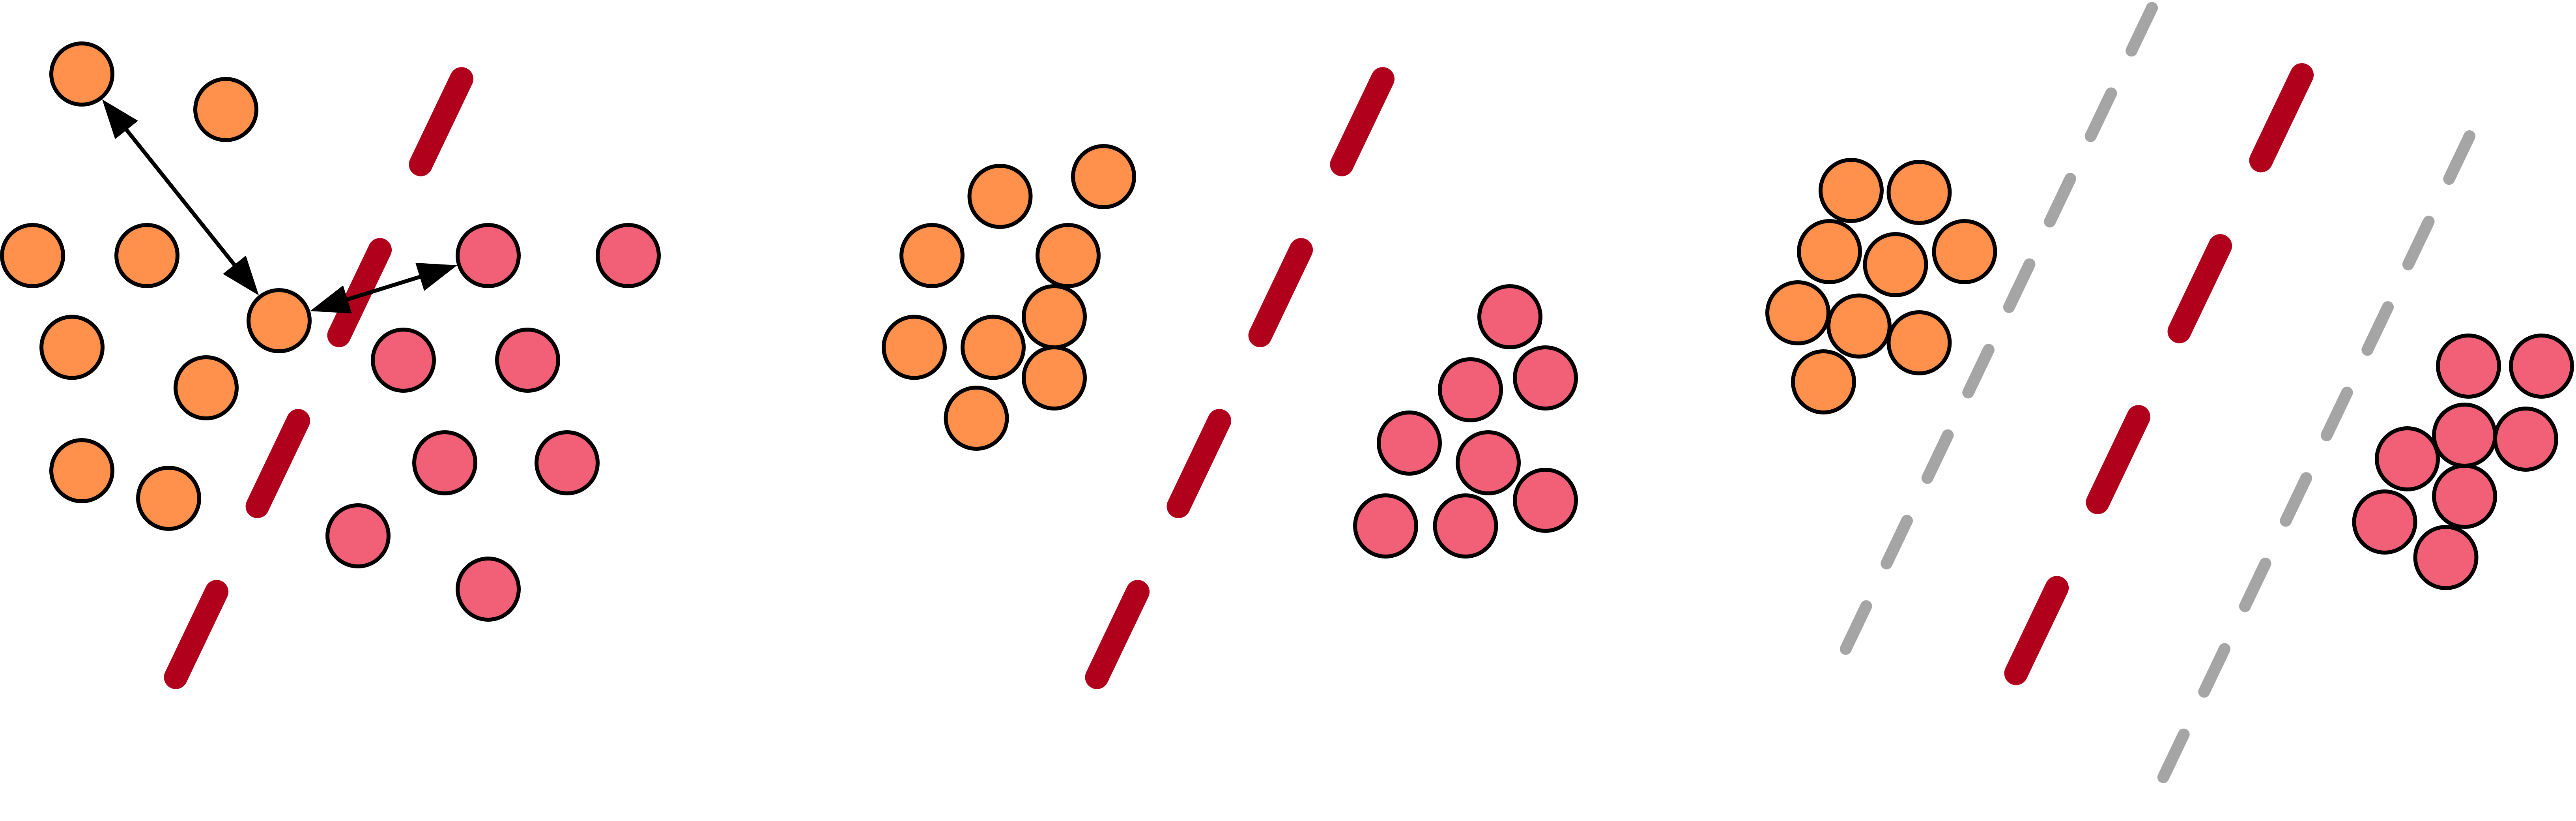
\includegraphics[height=3cm]{Img/c01_classification.png}
    \caption{度量学习和分类问题的区别}
    \label{classification}
\end{figure}
\par 如图\ref{classification}

\newpage

\subsection{多张图像插入示例}
\par 多张图像可以分别标记Label,方便后文引用.
\begin{figure}[!htbp]
    \centering
    \subfloat[Sigmoid函数与其梯度函数]{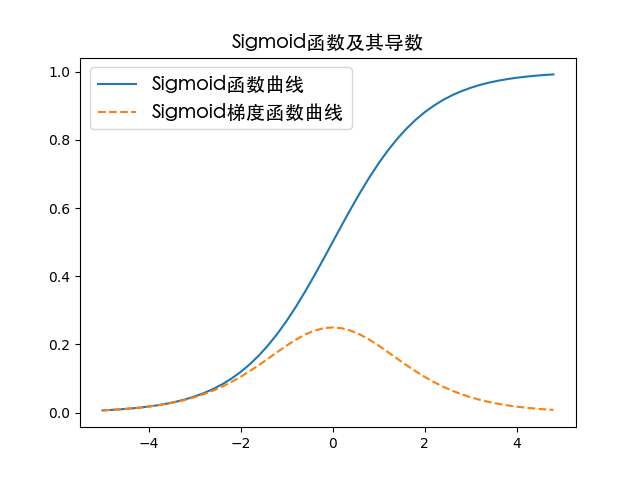
\includegraphics[width=0.5\textwidth]{Img/c01_sigmoid.png}}
    \hfill
    \subfloat[ReLU函数与其梯度函数]{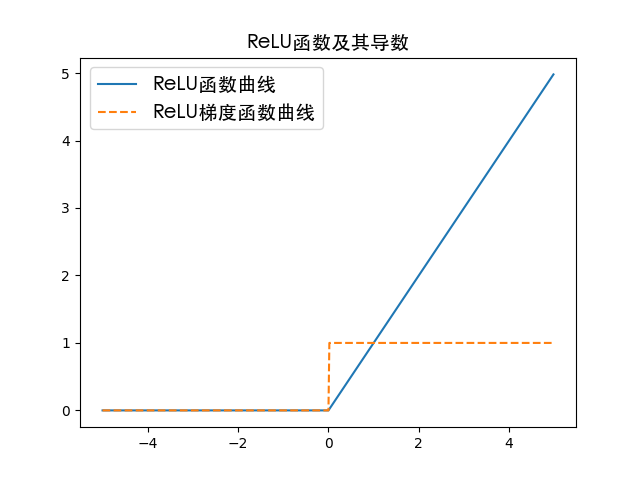
\includegraphics[width=0.5\textwidth]{Img/c01_ReLU.png}\label{relu}}
    \caption{常用的损失函数}    
    \label{activation function}
\end{figure}
\par 如图\ref{relu}.

\subsection{其他环境测试}
\begin{theorem} {这是一个定理.}
\end{theorem}
\begin{definition} {这是一个定义.}
\end{definition}
\begin{exam} {这是一个例子.}
\end{exam}
\begin{proof} {这是一个证明.}
\end{proof}
\begin{solution} {这是一个解.}
\end{solution}
{\chuhao 初号字.}\\
{\xiaochuhao 小初号字.}\\
{\yihao 一号字.}\\
{\erhao 二号字.}\\
{\xiaoerhao 小二号字.}\\
{\sanhao 三号字.}\\
{\sihao 四号字.}\\
{\xiaosihao 小四号字.}\\
{\wuhao 五号字.}\\
{\xiaowuhao 小五号字.}\\
{\liuhao 六号字.}\\
{\qihao 七号字.}\\
\par 公式
\begin{equation}
    \frac{\partial\mathcal{L}}{\partial x_i}=\frac{\frac{\partial\mathcal{L}}{\partial \Tilde{x_i}}-\Tilde{x_{i}}\sum_{j}\frac{\partial\mathcal{L}}{\partial \Tilde{x_j}}}{||x||_{2}}.\ 
\end{equation}
\newpage
\par 表格示例
\renewcommand{\arraystretch}{1.5} %控制行高
\setlength{\tabcolsep}{4mm}{
\begin{table}[!htbp]
		\scriptsize
		\centering
		\caption{部分模型在城市景观数据集上的表现}
		
		\label{Cityscapes}
		
\begin{tabular}{cccccc}
			
			\hline
			\toprule
			序号 & 模型框架 & 特征提取器 & Acc & mAcc & mIoU   \\ 		
			
			\midrule
			
			1 & FPN        & ResNet-50  & 95.81\% & 81.86\% & 74.51\% \\ 
			2 & FPN        & ResNet-101 & 96.01\% & 83.39\% & 75.80\% \\ 
			\midrule
			
			3 & PointRend  & ResNet-50  & 95.95\% & 84.05\% & 76.47\% \\ 
			4 & PointRend  & ResNet-101 & 96.23\% & 85.70\% & 78.30\% \\ 
			
			\midrule
			
			5 & DeeplabV3+ & ResNet-50  & 96.44\% & 86.96\% & 80.08\% \\ 
			6 & DeeplabV3+ & ResNet-101 & 96.57\% & 87.86\% & 80.97\% \\ 
			
			\bottomrule		
\end{tabular}	
\end{table}}
\newpage
